
\normalsize\chapter{METHODOLOGY }
\section{System Architecture}
\begin{figure}[H]
\centerline{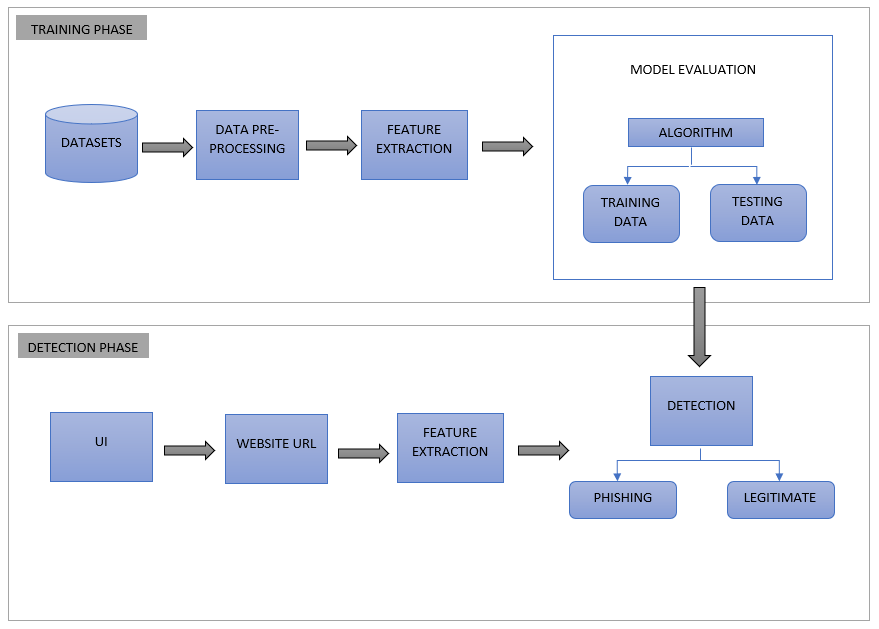
\includegraphics[scale=0.6]{newModel.png}}
\caption{System Architecture}
\label{fig}
\end{figure}
\par  In this section, we describe the phishing detection
framework which consists of two major parts as shown in Fig:3.1. The first part is the Training Phase and the second part is the Detection Phase. In
the first phase, datasets containing urls are prepared for the machine learning algorithm and model is evaluated. In the second phase, an input url is received from the user and based on the evaluated model, the url is classified into phishing or legitimate.
\section{Training Phase}
\subsection{Dataset}
\par  A dataset is a collection of structured or unstructured data that is organized and labeled for specific tasks. Datasets serve as the foundation for training and evaluating machine learning models, conducting statistical analysis, and extracting meaningful insights from data.
\par The dataset is created by merging two different datasets to improve the efficiency of prediction.
\begin{enumerate}
    \item Dataset-I
\par This dataset is collected from phishtank.com which contains 96,020 data with 50\% phishing and 50\% of legitimate urls. This dataset contains columns - domain and label,where domain represents the urls and label denotes whether the url is phishing or legitimate by representing 1 and 0 respectively.
    
    \item Dataset-II
\par This dataset is collected from Kaggle.com which contains 450,176 data, having url, label and result as columns.
\end{enumerate}
\begin{figure}[H]
\centerline{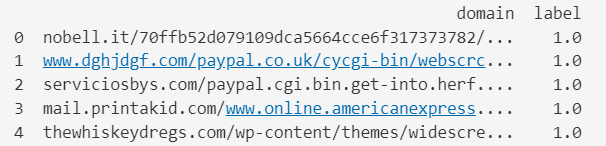
\includegraphics[scale=0.8]{dataset1.png}}
\caption{Dataset-I from phishtank.com}
\label{fig}
\end{figure}
\begin{figure}[H]
\centerline{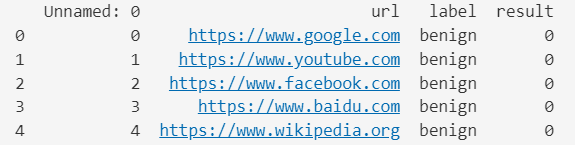
\includegraphics[scale=0.8]{dataset2.png}}
\caption{Dataset-II from kaggle.com}
\label{fig}
\end{figure}

\subsection{Data Pre-Processing}
\par
Data preprocessing is a crucial step in machine learning that involves transforming raw data into a suitable format for training machine learning models. It helps to improve the quality and reliability of the data, reduces noise and inconsistencies, and enhances the performance of the models.Here are some data preprocessing techniques used in our project :
\begin{enumerate}
  \item Data Cleaning: This step involves handling missing values, outliers, and duplicates in the data. Missing values can be imputed using techniques like mean, median, or mode. Outliers can be detected and treated using statistical methods or replaced with more reasonable values. Duplicates can be removed to avoid bias in the analysis.
  \item Data Reduction: Data reduction in preprocessing refers to the process of reducing the size or complexity of a dataset without losing critical information. It is often performed as an initial step in data preprocessing to address challenges such as computational limitations, storage constraints, or noise in the data. Data reduction techniques aim to retain the most relevant information while reducing redundancy and removing irrelevant or noisy data points. 
  \item Data Integration: Data integration in preprocessing refers to the process of combining multiple heterogeneous data sources into a unified and consistent format. It involves merging, transforming, and resolving inconsistencies in the data from different sources to create a comprehensive dataset for further analysis or modeling. Data integration is a critical step in data preprocessing when working with data from various systems, databases, or file formats. 
  
\end{enumerate}
\subsection{Feature Extraction}
\par Feature extraction in machine learning refers to the process of transforming raw input data into a set of meaningful and representative features that can be used as inputs for machine learning algorithms. The goal of feature extraction is to capture relevant information from the data and create a compact and informative representation that facilitates the learning process and improves the performance of the models.
\par Statistical measures can be computed from the raw data to capture important characteristics. These measures can include mean, median, standard deviation, variance, skewness, kurtosis, and other moments. Statistical measures provide insights into the distribution, central tendency, and spread of the data. Exploratory data analysis, domain expertise, and experimentation are often necessary to determine the most effective feature extraction methods for a given problem.
\par In this project, the features are classified into 2 categories:
\begin{itemize}
    \item Lexical Features
    \item Numerical Features
\end{itemize}

\subsection{Algorithm}

\subsubsection{Logistic Regression}
\par Logistic regression is a statistical modeling technique used for binary classification problems, where the goal is to predict the probability of an event or the likelihood of an outcome falling into one of two classes. Despite its name, logistic regression is a classification algorithm rather than a regression algorithm. It is based on the assumption that the relationship between the input variables (also known as independent or predictor variables) and the log-odds of the binary outcome (dependent or response variable) can be approximated by a linear relationship.
\par The logistic function, also called the sigmoid function, is used to map the linear combination of input variables to a range between 0 and 1, representing the probability of belonging to the positive class. The logistic function is given by:

p(x) = 1 / (1 + e\^(-z))

where p(x) is the predicted probability, x is the input variables, and z is the linear combination of the input variables.
\begin{figure}[H]
\centerline{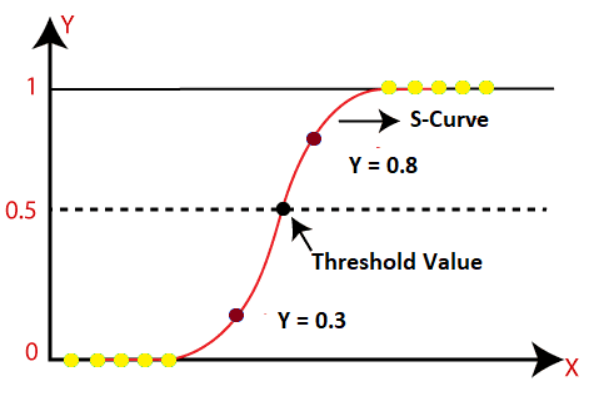
\includegraphics[scale=0.8]{LRgraph.png}}
\caption{Logistic Regression}
\label{fig}
\end{figure}
\section{Detection Phase}
\subsection{User Interface}
\par A user interface (UI) refers to the visual and interactive elements through which users interact with a software application or system. It provides a means for users to input commands or data and receive feedback or output from the system. The primary goal of a user interface is to create a user-friendly and intuitive experience, allowing users to efficiently and effectively interact with the software.
\subsubsection{Reactjs}
\par ReactJS, also known as React, is a popular JavaScript library for building user interfaces. It was developed by Facebook and is widely used for creating interactive and dynamic web applications. React follows a component-based architecture, where the UI is broken down into reusable and modular components, making it easier to develop and maintain complex user interfaces.
\subsubsection{Nodejs}
\par Node.js is an open-source JavaScript runtime environment built on Chrome's V8 JavaScript engine. It allows developers to run JavaScript code outside the browser, on the server-side, and build scalable and high-performance web applications. Node.js provides an event-driven, non-blocking I/O model that makes it lightweight and efficient, suitable for real-time applications and server-side programming.
\par Node.js can be used to build APIs (Application Programming Interfaces) for server-side development. APIs are used to define the endpoints and functionality of web services, allowing client applications to interact with the server and exchange data.

\subsection{Website URL}
\par A URL (Uniform Resource Locator) is a specific address that identifies a resource on the internet. It typically consists of several components, including the protocol, domain name, path, and possibly query parameters.
\begin{figure}[H]
\centerline{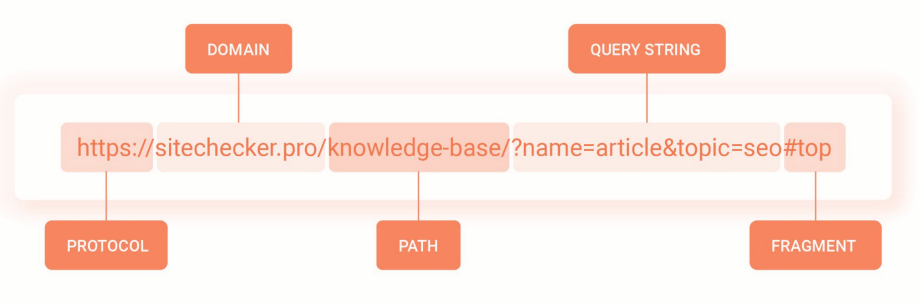
\includegraphics[scale=0.6]{features.png}}
\caption{Basic structure of a URL}
\label{fig}
\end{figure}

\subsection{Detection}
\par The input URL from the user interface is predicted either as Phishing or Non-Phishing.
\begin{itemize}
    \item Phishing: Type of URLs that are specifically designed to deceive users by impersonating legitimate websites or services.
    \item Non-Phishing Type of URLs that are the genuine URLs of legitimate websites or services.
\end{itemize}

\section{Objectives}

\begin{itemize}
    \item To extract features that can produce effective accuracy in model evaluation
\item To analyse the accuracy level for different machine learning algorithms and implementing the best among them
\item To design and Implement a Web Application to search and detect whether it is phishing or not.
\item To store URLs, which are detected as either phishing or non-phishing

\end{itemize}
\section{Scope}
\begin{itemize}
    \item Algorithm will analyze various blacklisted and legitimate URL features to accurately detect the phishing websites including zero-hour phishing websites.

\end{itemize}

\section{System Requirements}
\subsection{  Software Requirements  }
\renewcommand{\labelitemi}{}

\begin{itemize}
    \item \textbf{Programming Languages:} Python, JavaScript
    \item \textbf{Integrated Development Environment (IDE):}VisualStudioCode, Google Colab
    \item \textbf{Libraries:} numpy, panda, scikit-learn, Matplotlib/Seaborn, pycaret, pickle, React
    \item \textbf{Frameworks:} Anaconda, Express.js
    \item \textbf{Web Browsers:} Google Chrome, Mozilla Firefox,Microsoft Edge
    \item \textbf{Package Managers:} pip, npm
    \item \textbf{Version Control:} Git, Github
\end{itemize}


\subsection{Hardware Requirements}
\begin{itemize}
    \item \textbf{Processor:} Intel i5 and above
    \item \textbf{RAM:} 8gb and above
\end{itemize}





















